\documentclass{article}

% content/resources/templates/preamble.tex
\usepackage[margin=0.6in]{geometry}
\author{Milav Dabgar}
\usepackage{amsmath,amssymb,amsthm}
\usepackage{booktabs}
\usepackage{multirow}
\usepackage{xcolor}
\usepackage{tcolorbox}
\tcbuselibrary{breakable,skins}
\usepackage[colorlinks=true,linkcolor=blue]{hyperref}
\usepackage{titlesec}
\usepackage{enumitem}
\usepackage{tikz}
\usepackage{pgfplots}
\usepackage{circuitikz}
\usepackage[version=4]{mhchem}
\usepackage{longtable}
\usepackage{array}
\usepackage{float}
\usepackage{caption}
\usepackage{listings}

\lstset{
  basicstyle=\small\ttfamily,
  breaklines=true,
  breakatwhitespace=false,
  postbreak=\mbox{\textcolor{red}{$\hookrightarrow$}\space},
  float=false,
  numbers=left,
  numberstyle=\tiny\color{gray},
  numbersep=10pt,
  xleftmargin=2em,
  keywordstyle=\color{blue},
  commentstyle=\color{green!60!black},
  stringstyle=\color{purple},
  backgroundcolor=\color{gray!5},
  showstringspaces=false,
  tabsize=2,
  captionpos=b,
  keepspaces=true,
  columns=flexible
}

\pgfplotsset{compat=1.18}
\usetikzlibrary{shapes,arrows,positioning,calc,patterns,decorations.pathmorphing,decorations.markings,arrows.meta}

% Color scheme
\definecolor{headcolor}{RGB}{0,102,204}
\definecolor{keycolor}{RGB}{220,20,60}
\definecolor{solutioncolor}{RGB}{34,139,34}
\definecolor{mnemoniccolor}{RGB}{148,0,211}
\definecolor{codecolor}{RGB}{0,0,100}

% Spacing
\setlength{\parskip}{3pt}
\setlist[itemize]{nosep}
\setlist[enumerate]{nosep}

% Title formatting
\titleformat{\section}{\Large\bfseries\color{headcolor}}{\thesection}{1em}{}
\titleformat{\subsection}{\large\bfseries\color{headcolor}}{\thesubsection}{1em}{}

% Pandoc tightlist compatibility
\providecommand{\tightlist}{%
  \setlength{\itemsep}{0pt}\setlength{\parskip}{0pt}}

% Pandoc longtable compatibility
\newcounter{none}
\def\thenone{}


% content/resources/templates/english-boxes.tex

% Custom environments
\newtcolorbox{solutionbox}{
 breakable,
 enhanced,
 colback=solutioncolor!5!white,
 colframe=solutioncolor!75!black,
 fonttitle=\bfseries,
 title=Solution
}

\newtcolorbox{solutionboxnobreak}{
 colback=solutioncolor!5!white,
 colframe=solutioncolor!75!black,
 fonttitle=\bfseries,
 title=Solution
}

\newtcolorbox{keyformula}{
 breakable,
 enhanced,
 colback=keycolor!5!white,
 colframe=keycolor!75!black,
 fonttitle=\bfseries,
 title=Key Formula
}

\newtcolorbox{mnemonicboxenv}{
 breakable,
 enhanced,
 colback=mnemoniccolor!5!white,
 colframe=mnemoniccolor!75!black,
 fonttitle=\bfseries,
 title=Mnemonic
}

\newcommand{\mnemonicbox}[1]{%
  \begin{mnemonicboxenv}
    #1
  \end{mnemonicboxenv}
}


% Custom commands for GTU solutions
% This file defines semantic commands for consistent formatting

% Question command with automatic formatting
\newcommand{\question}[2]{%
  \section*{Question #1}%
  \textbf{#2}%
}

% OR question variant
\newcommand{\questionor}[2]{%
  \section*{Question #1 OR}%
  \textbf{#2}%
}

% Proper table environment with caption
\newenvironment{answertable}[1]{%
  \begin{table}[htbp]
  \centering
  \caption{#1}
}{%
  \end{table}
}

% Proper figure environment for diagrams
\newenvironment{answerdiagram}[1]{%
  \begin{figure}[htbp]
  \centering
  \caption{#1}
}{%
  \end{figure}
}

% Semantic markup for key terms
\newcommand{\keyword}[1]{\textbf{#1}}
\newcommand{\code}[1]{\texttt{#1}}
\newcommand{\classname}[1]{\texttt{#1}}
\newcommand{\methodname}[1]{\texttt{#1}}

% Proper quotation marks
\newcommand{\mnemonic}[1]{``#1''}

\usetikzlibrary{mindmap,trees,shadows}

\title{Database Management System (1333204) - Summer 2024 Solution}
\date{June 14, 2024}

\begin{document}
\maketitle

\questionmarks{1(a)}{3}{Define: DBMS, Instance, Metadata}

\begin{solutionbox}

\begin{itemize}
    \item \textbf{DBMS (Database Management System)}: Software that enables users to create, maintain, and access databases by controlling data organization, storage, retrieval, security, and integrity.
    \item \textbf{Instance}: The actual data stored in a database at a particular moment in time. It's the current state or snapshot of a database.
    \item \textbf{Metadata}: Data about data that describes database structure, including tables, fields, relationships, constraints, and indexes.
\end{itemize}

\end{solutionbox}

\begin{mnemonicbox}[title={DIM view}]Database system, Instance snapshot, Metadata description\end{mnemonicbox}

\questionmarks{1(b)}{4}{Define and Explain with example: 1.Entity 2. Attribute}

\begin{solutionbox}

\textbf{Table: Entity vs Attribute}

\begin{table}[H]
    \centering
    \begin{tabulary}{\linewidth}{|L|L|L|}
    \hline
    \textbf{Concept} & \textbf{Definition} & \textbf{Example} \\
    \hline
    Entity & A real-world object or concept that can be distinctly identified & Student (John), Book (Harry Potter), Car (Toyota Camry) \\
    \hline
    Attribute & Characteristic or property that describes an entity & Student: roll\_no, name, address \newline Book: ISBN, title, author \\
    \hline
    \end{tabulary}
\end{table}

\textbf{Diagram:}

\begin{center}
\begin{tikzpicture}
    % Student Entity
    \node[gtu block] (std) {
        \textbf{STUDENT} \\
        \par\noindent\rule{3cm}{0.4pt}\par
        + student\_id \\
        + name \\
        + address
    };
    
    % Book Entity
    \node[gtu block, right=3cm of std] (book) {
        \textbf{BOOK} \\
        \par\noindent\rule{3cm}{0.4pt}\par
        + ISBN \\
        + title \\
        + author
    };
\end{tikzpicture}
\end{center}

\end{solutionbox}

\begin{mnemonicbox}[title={EA-PC}]Entities Are Physical/Conceptual, Attributes Provide Characteristics\end{mnemonicbox}

\questionmarks{1(c)}{7}{Write the full form of DBA. Explain the roles and responsibilities of DBA.}

\begin{solutionbox}

DBA stands for \textbf{Database Administrator}.

\textbf{Table: DBA Responsibilities}

\begin{table}[H]
    \centering
    \begin{tabulary}{\linewidth}{|L|L|}
    \hline
    \textbf{Role} & \textbf{Description} \\
    \hline
    Database Design & Creates logical/physical database structure and schema \\
    \hline
    Security Management & Controls access through user accounts and permissions \\
    \hline
    Performance Tuning & Optimizes queries, indexes for faster data retrieval \\
    \hline
    Backup \& Recovery & Implements strategies to prevent data loss \\
    \hline
    Maintenance & Updates software, applies patches, monitors space \\
    \hline
    \end{tabulary}
\end{table}

\textbf{Diagram:}

\begin{center}
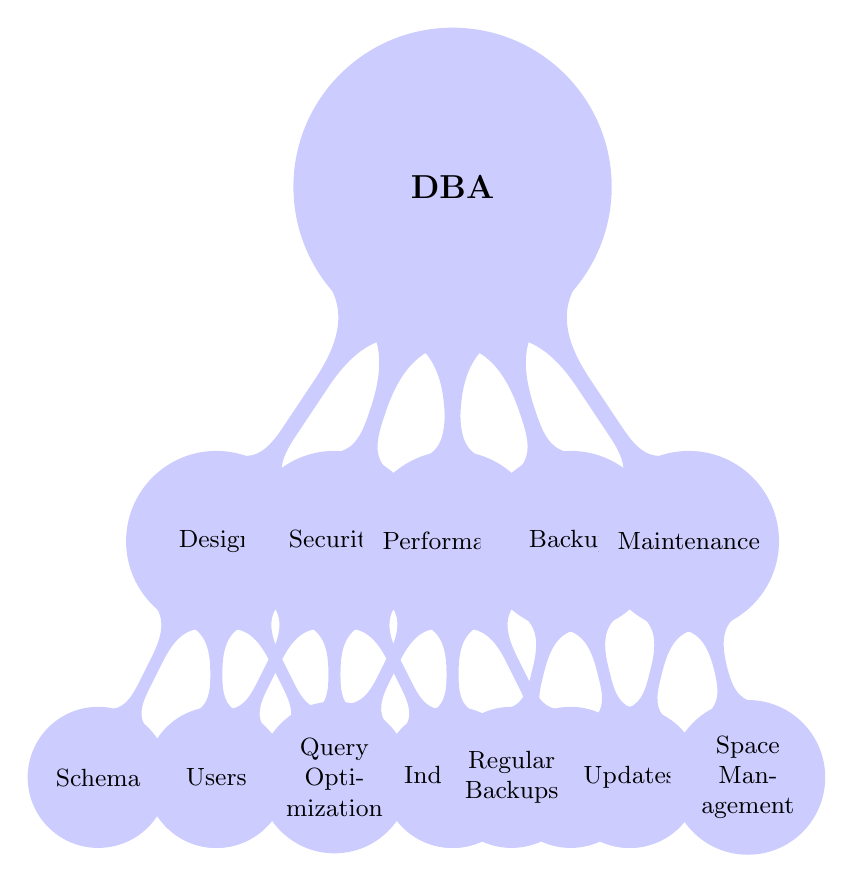
\begin{tikzpicture}[
    mindmap,
    concept color=blue!20,
    every node/.style={concept},
    root concept/.append style={font=\large\bfseries},
    level 1/.append style={level distance=4.5cm, sibling angle=72},
    level 2/.append style={level distance=3cm, sibling angle=45, font=\small}
]
    \node[root concept] {DBA}
        child { node {Design}
            child { node {Schema} }
            child { node {Tables} }
            child { node {Relationships} }
        }
        child { node {Security}
            child { node {Users} }
            child { node {Permissions} }
            child { node {Encryption} }
        }
        child { node {Performance}
            child { node {Query Optimization} }
            child { node {Indexing} }
            child { node {Monitoring} }
        }
        child { node {Backup}
            child { node {Regular Backups} }
            child { node {Recovery Plans} }
        }
        child { node {Maintenance}
            child { node {Updates} }
            child { node {Space Management} }
        };
\end{tikzpicture}
\end{center}

\end{solutionbox}

\begin{mnemonicbox}[title={SPMBU}]Security, Performance, Maintenance, Backup, Updates\end{mnemonicbox}

\questionmarks{1(c) OR}{7}{Explain relational and network data models in detail.}

\begin{solutionbox}

\textbf{Table: Relational vs Network Data Models}

\begin{table}[H]
    \centering
    \begin{tabulary}{\linewidth}{|L|L|L|}
    \hline
    \textbf{Feature} & \textbf{Relational Model} & \textbf{Network Model} \\
    \hline
    Structure & Tables (relations) with rows and columns & Records connected by pointers forming complex networks \\
    \hline
    Relationship & Related through primary \& foreign keys & Direct links between parent-child records \\
    \hline
    Flexibility & High - tables can be joined as needed & Limited - predefined physical connections \\
    \hline
    Examples & MySQL, Oracle, SQL Server & IDS, IDMS \\
    \hline
    Query Language & SQL (structured query language) & Procedural languages \\
    \hline
    \end{tabulary}
\end{table}

\textbf{Diagram:}

\begin{center}
\begin{tikzpicture}
    % Relational Model
    \node (rel_label) {\textbf{Relational Model}};
    
    \node[gtu block, below=0.5cm of rel_label] (courses) {Table: Courses};
    \node[gtu block, left=0.5cm of courses] (students) {Table: Students};
    \node[gtu block, right=0.5cm of courses] (grades) {Table: Grades};
    
    \draw (students) -- (grades);
    \draw (courses) -- (grades);
    
    % Network Model
    \node[right=6cm of rel_label] (net_label) {\textbf{Network Model}};
    
    \node[gtu block, below=0.5cm of net_label] (rec_student) {Record: Student};
    \node[gtu block, below left=1cm and -0.5cm of rec_student] (rec_c1) {Record: Course1};
    \node[gtu block, below right=1cm and -0.5cm of rec_student] (rec_c2) {Record: Course2};
    \node[gtu block, below=1cm of rec_c2] (rec_grade) {Record: Grade};
    
    \draw[gtu arrow] (rec_student) -- (rec_c1);
    \draw[gtu arrow] (rec_student) -- (rec_c2);
    \draw[gtu arrow] (rec_c2) -- (rec_grade);
\end{tikzpicture}
\end{center}

\end{solutionbox}

\begin{mnemonicbox}[title={RSPEN}]Relational uses Sets, Pointers Enable Networks\end{mnemonicbox}

\questionmarks{2(a)}{3}{Draw figure and Explain Generalization.}

\begin{solutionbox}

\textbf{Generalization}: The process of extracting common characteristics from two or more entities to create a new higher-level entity.

\textbf{Diagram:}

\begin{center}
\begin{tikzpicture}[node distance=2cm]
    \node[gtu block] (vehicle) {
        \textbf{Vehicle} \\
        + vehicle\_id \\
        + manufacturer \\
        + year
    };
    
    \node[gtu block, below left=2cm and 1cm of vehicle] (car) {
        \textbf{Car} \\
        + num\_doors \\
        + fuel\_type
    };
    
    \node[gtu block, below=2cm of vehicle] (truck) {
        \textbf{Truck} \\
        + cargo\_capacity \\
        + towing\_capacity
    };
    
    \node[gtu block, below right=2cm and 1cm of vehicle] (moto) {
        \textbf{Motorcycle} \\
        + engine\_size \\
        + type
    };
    
    % Inheritance arrows
    \draw[gtu arrow, -{Triangle[open, scale=2]}] (car) -- (vehicle);
    \draw[gtu arrow, -{Triangle[open, scale=2]}] (truck) -- (vehicle);
    \draw[gtu arrow, -{Triangle[open, scale=2]}] (moto) -- (vehicle);
\end{tikzpicture}
\end{center}

\end{solutionbox}

\begin{mnemonicbox}[title={BUSH}]Bottom-Up Shared Hierarchy\end{mnemonicbox}

\questionmarks{2(b)}{4}{Explain Primary Key and Foreign Key Constraints.}

\begin{solutionbox}

\textbf{Table: Primary Key vs Foreign Key}

\begin{table}[H]
    \centering
    \begin{tabulary}{\linewidth}{|L|L|L|L|}
    \hline
    \textbf{Constraint} & \textbf{Definition} & \textbf{Properties} & \textbf{Example} \\
    \hline
    Primary Key & Uniquely identifies each record in a table & Unique, Not Null, Only one per table & StudentID in Students table \\
    \hline
    Foreign Key & Links data between tables, references a primary key in another table & Can be NULL, Multiple allowed per table & DeptID in Employees table referencing Departments table \\
    \hline
    \end{tabulary}
\end{table}

\textbf{Diagram:}

\begin{center}
\begin{tikzpicture}[node distance=4cm]
    \node[gtu block] (dept) {
        \textbf{DEPARTMENT} \\
        + \underline{dept\_id} PK \\
        + dept\_name
    };
    
    \node[gtu block, right=of dept] (emp) {
        \textbf{EMPLOYEE} \\
        + \underline{emp\_id} PK \\
        + name \\
        + dept\_id FK
    };
    
    \draw[gtu arrow] (dept) -- node[above] {1} node[below] {has} (emp);
    \node[above left] at (emp.west) {M};
\end{tikzpicture}
\end{center}

\end{solutionbox}

\begin{mnemonicbox}[title={PURE FIRE}]Primary Uniquely References Entities, Foreign Imports Referenced Entities\end{mnemonicbox}

\questionmarks{2(c)}{7}{Construct an E-R diagram for Hospital Management System.}

\begin{solutionbox}

\textbf{E-R Diagram for Hospital Management System:}

\begin{center}
\begin{tikzpicture}[node distance=2.5cm, every node/.style={scale=0.8}, transform shape]
    % Entities with attributes
    \node[gtu block] (patient) {
        \textbf{PATIENT} \\
        + \underline{patient\_id} PK \\
        + name, address \\
        + DOB, phone
    };
    
    \node[gtu block, right=4cm of patient] (doc) {
        \textbf{DOCTOR} \\
        + \underline{doctor\_id} PK, name \\
        + specialization \\
        + dept\_id FK
    };
    
    \node[gtu block, below=3cm of patient] (room) {
        \textbf{ROOM} \\
        + \underline{room\_id} PK \\
        + type \\
        + availability
    };
    
    \node[gtu block, below=3cm of doc] (app) {
        \textbf{APPOINTMENT} \\
        + \underline{app\_id} PK \\
        + patient\_id FK \\
        + doctor\_id FK \\
        + date\_time, status
    };
    
    \node[gtu block, right=3cm of doc] (dept) {
        \textbf{DEPARTMENT} \\
        + \underline{dept\_id} PK \\
        + name \\
        + location
    };
    
    \node[gtu block, below=2cm of app] (pres) {
        \textbf{PRESCRIPTION} \\
        + \underline{pres\_id} PK \\
        + app\_id FK \\
        + date \\
        + medications
    };
    
    % Relationships
    \draw[gtu arrow] (patient) -- node[midway, fill=white] {makes} (app);
    \draw[gtu arrow] (doc) -- node[midway, fill=white] {conducts} (app);
    \draw[gtu arrow] (app) -- node[midway, fill=white] {generates} (pres);
    \draw[gtu arrow] (dept) -- node[midway, fill=white] {employs} (doc);
    \draw[gtu arrow] (room) -- node[midway, fill=white] {admits} (patient);
    
\end{tikzpicture}
\end{center}

\end{solutionbox}

\begin{mnemonicbox}[title={PADRE}]Patients Appointments Doctors Rooms Entities\end{mnemonicbox}

\questionmarks{2(a) OR}{3}{Draw figure and Explain Specialization.}

\begin{solutionbox}

\textbf{Specialization}: The process of creating new entities from an existing entity by adding unique attributes to distinguish them.

\textbf{Diagram:}

\begin{center}
\begin{tikzpicture}[node distance=2cm]
    \node[gtu block] (emp) {
        \textbf{Employee} \\
        + emp\_id \\
        + name \\
        + address \\
        + phone
    };
    
    \node[gtu block, below left=2cm and 1cm of emp] (full) {
        \textbf{FullTime} \\
        + salary \\
        + benefits
    };
    
    \node[gtu block, below right=2cm and 1cm of emp] (part) {
        \textbf{PartTime} \\
        + hourly\_rate \\
        + hours\_worked
    };
    
    % Specialization arrows (Top-down)
    \draw[gtu arrow] (emp) -- (full);
    \draw[gtu arrow] (emp) -- (part);
\end{tikzpicture}
\end{center}

\end{solutionbox}

\begin{mnemonicbox}[title={TDSB}]Top-Down Specialized Breakdown\end{mnemonicbox}

\questionmarks{2(b) OR}{4}{Explain single valued v/s multi-valued attributes with suitable examples.}

\begin{solutionbox}

\textbf{Table: Single-valued vs Multi-valued Attributes}

\begin{table}[H]
    \centering
    \begin{tabulary}{\linewidth}{|L|L|L|L|}
    \hline
    \textbf{Type} & \textbf{Definition} & \textbf{Example} & \textbf{Implementation} \\
    \hline
    Single-valued & Contains only one value for each entity instance & Person's birth date, SSN & Directly stored in table columns \\
    \hline
    Multi-valued & Can have multiple values for the same entity & Person's skills, phone numbers & Separate table or specialized formats \\
    \hline
    \end{tabulary}
\end{table}

\textbf{Diagram:}

\begin{center}
\begin{tikzpicture}[node distance=4cm]
    \node[gtu block] (emp) {
        \textbf{EMPLOYEE} \\
        + emp\_id \\
        + name \\
        + birth\_date (Single)
    };
    
    \node[gtu block, right=of emp, yshift=1.5cm] (phone) {
        \textbf{PHONE\_NUMBERS} \\
        + emp\_id \\
        + phone\_number (Multi)
    };
    
    \node[gtu block, right=of emp, yshift=-1.5cm] (skill) {
        \textbf{SKILLS} \\
        + emp\_id \\
        + skill (Multi)
    };
    
    \draw[gtu arrow] (emp) -- node[midway, fill=white] {has} (phone);
    \draw[gtu arrow] (emp) -- node[midway, fill=white] {possesses} (skill);
\end{tikzpicture}
\end{center}

\end{solutionbox}

\begin{mnemonicbox}[title={SOME}]Single One, Multiple Entries\end{mnemonicbox}

\questionmarks{2(c) OR}{7}{Construct an E-R diagram for Banking Management System.}

\begin{solutionbox}

\textbf{E-R Diagram for Banking Management System:}

\begin{center}
\begin{tikzpicture}[node distance=3cm, every node/.style={scale=0.85}, transform shape]
    \node[gtu block] (customer) {
        \textbf{CUSTOMER} \\
        + \underline{customer\_id} PK \\
        + name, address, phone, email
    };
    
    \node[gtu block, right=4cm of customer] (account) {
        \textbf{ACCOUNT} \\
        + \underline{account\_no} PK \\
        + customer\_id FK \\
        + branch\_id FK \\
        + balance, type
    };
    
    \node[gtu block, below=2cm of customer] (loan) {
        \textbf{LOAN} \\
        + \underline{loan\_id} PK \\
        + customer\_id FK \\
        + amount, interest
    };
    
    \node[gtu block, below=2cm of account] (trans) {
        \textbf{TRANSACTION} \\
        + \underline{trans\_id} PK \\
        + account\_no FK \\
        + date, amount, type
    };
    
    \node[gtu block, right=4cm of account] (branch) {
        \textbf{BRANCH} \\
        + \underline{branch\_id} PK \\
        + name, location
    };
    
    \node[gtu block, below=2cm of branch] (emp) {
        \textbf{EMPLOYEE} \\
        + \underline{emp\_id} PK \\
        + name, position, salary \\
        + branch\_id FK
    };
    
    % Relationships
    \draw[gtu arrow] (customer) -- node[midway, fill=white] {owns} (account);
    \draw[gtu arrow] (customer) -- node[midway, fill=white] {takes} (loan);
    \draw[gtu arrow] (account) -- node[midway, fill=white] {has} (trans);
    \draw[gtu arrow] (branch) -- node[midway, fill=white] {maintains} (account);
    \draw[gtu arrow] (branch) -- node[midway, fill=white] {works\_at} (emp);
    
\end{tikzpicture}
\end{center}

\end{solutionbox}

\begin{mnemonicbox}[title={CABLE}]Customers Accounts Branches Loans Employees\end{mnemonicbox}

\questionmarks{3(a)}{3}{Explain WHERE and DESC clause with example.}

\begin{solutionbox}

\textbf{Table: WHERE and DESC Clauses}

\begin{table}[H]
    \centering
    \begin{tabulary}{\linewidth}{|L|L|L|L|}
    \hline
    \textbf{Clause} & \textbf{Purpose} & \textbf{Syntax} & \textbf{Example} \\
    \hline
    WHERE & Filters rows based on specified condition & SE... FROM ... WHERE condition & SELECT * FROM employees WHERE salary > 50000 \\
    \hline
    DESC & Sorts results in descending order & SE... ORDER BY ... DESC & SELECT * FROM products ORDER BY price DESC \\
    \hline
    \end{tabulary}
\end{table}

\textbf{Diagram (Data Flow):}

\begin{lstlisting}[language=sql, title={Example Data Operation}]
-- Original
| ID | Name   | Marks |
| 1  | Alice  | 85    |
| 2  | Bob    | 92    |
| 3  | Carol  | 78    |

-- WHERE Marks > 80
| 1  | Alice  | 85    |
| 2  | Bob    | 92    |

-- ORDER BY Marks DESC
| 2  | Bob    | 92    |
| 1  | Alice  | 85    |
| 3  | Carol  | 78    |
\end{lstlisting}

\end{solutionbox}

\begin{mnemonicbox}[title={WDF}]Where filters Data, DESC orders First-highest\end{mnemonicbox}

\questionmarks{3(b)}{4}{List DDL commands. Explain any two DDL commands with examples.}

\begin{solutionbox}

\textbf{DDL (Data Definition Language) Commands:}
\begin{enumerate}
    \item CREATE
    \item ALTER
    \item DROP
    \item TRUNCATE
    \item RENAME
\end{enumerate}

\textbf{Table: CREATE and ALTER Commands}

\begin{table}[H]
    \centering
    \begin{tabulary}{\linewidth}{|L|L|L|L|}
    \hline
    \textbf{Command} & \textbf{Purpose} & \textbf{Syntax} & \textbf{Example} \\
    \hline
    CREATE & Creates database objects & CREATE TABLE ... & CREATE TABLE students (id INT...) \\
    \hline
    ALTER & Modifies structure & ALTER TABLE ... & ALTER TABLE students ADD COLUMN... \\
    \hline
    \end{tabulary}
\end{table}

\begin{lstlisting}[language=sql]
-- CREATE example
CREATE TABLE employees (
    emp_id INT PRIMARY KEY,
    name VARCHAR(50) NOT NULL,
    dept VARCHAR(30),
    salary DECIMAL(10,2)
);

-- ALTER example
ALTER TABLE employees 
ADD COLUMN hire_date DATE;
\end{lstlisting}

\end{solutionbox}

\begin{mnemonicbox}[title={CADTR}]Create Alter Drop Truncate Rename\end{mnemonicbox}

\questionmarks{3(c)}{7}{Perform the following Query on the table "Company" having the field's eno, ename, salary, dept in SQL.}

\textbf{Queries:}
\begin{enumerate}
    \item Display all records in Company table.
    \item Display only dept without duplicate value.
    \item Display all records sorted in descending order of ename.
    \item Add one new column "cityname" to store city.
    \item Display name of all employees who do not stay in city "Mumbai".
    \item Delete all employees having salary less than 10,000.
    \item Display the employee names starts with "A".
\end{enumerate}

\begin{solutionbox}

\begin{lstlisting}[language=sql]
-- 1. Display all records
SELECT * FROM Company;

-- 2. Display only dept without duplicates
SELECT DISTINCT dept FROM Company;

-- 3. Display records sorted by ename descending
SELECT * FROM Company ORDER BY ename DESC;

-- 4. Add new column "cityname"
ALTER TABLE Company ADD COLUMN cityname VARCHAR(50);

-- 5. Employees not in Mumbai
SELECT ename FROM Company WHERE cityname != 'Mumbai';

-- 6. Delete employees with salary < 10000
DELETE FROM Company WHERE salary < 10000;

-- 7. Employee names starting with "A"
SELECT ename FROM Company WHERE ename LIKE 'A%';
\end{lstlisting}

\textbf{Table: SQL Operations}

\begin{table}[H]
    \centering
    \begin{tabulary}{\linewidth}{|L|L|L|}
    \hline
    \textbf{Operation} & \textbf{SQL Command} & \textbf{Purpose} \\
    \hline
    SELECT & SELECT * FROM Company & Retrieve all data \\
    \hline
    DISTINCT & SELECT DISTINCT dept & Remove duplicates \\
    \hline
    ORDER BY & ORDER BY ename DESC & Sort in descending \\
    \hline
    ALTER & ALTER TABLE ADD COLUMN & Add new column \\
    \hline
    WHERE & WHERE cityname != 'Mumbai' & Filter condition \\
    \hline
    DELETE & DELETE FROM WHERE & Remove records \\
    \hline
    LIKE & WHERE ename LIKE 'A\%' & Pattern matching \\
    \hline
    \end{tabulary}
\end{table}

\end{solutionbox}

\begin{mnemonicbox}[title={SODA-WDL}]Select Order Distinct Alter - Where Delete Like\end{mnemonicbox}

\questionmarks{3(a) OR}{3}{Explain SELECT and DISTINCT clause with example.}

\begin{solutionbox}

\textbf{Table: SELECT and DISTINCT Clauses}

\begin{table}[H]
    \centering
    \begin{tabulary}{\linewidth}{|L|L|L|L|}
    \hline
    \textbf{Clause} & \textbf{Purpose} & \textbf{Syntax} & \textbf{Example} \\
    \hline
    SELECT & Retrieves data from database & SELECT columns FROM table & SELECT name, age FROM students \\
    \hline
    DISTINCT & Eliminates duplicate values & SELECT DISTINCT columns FROM table & SELECT DISTINCT department FROM employees \\
    \hline
    \end{tabulary}
\end{table}

\begin{lstlisting}[language=sql]
-- Original: Sales, IT, HR, IT, Sales

-- SELECT dept_name
Sales
IT
HR
IT
Sales

-- SELECT DISTINCT dept_name
Sales
IT
HR
\end{lstlisting}

\end{solutionbox}

\begin{mnemonicbox}[title={SUD}]Select Unique with Distinct\end{mnemonicbox}

\questionmarks{3(b) OR}{4}{List DML commands. Explain any two DML commands with examples.}

\begin{solutionbox}

\textbf{DML (Data Manipulation Language) Commands:}
\begin{enumerate}
    \item INSERT
    \item UPDATE
    \item DELETE
    \item SELECT
\end{enumerate}

\textbf{Table: INSERT and UPDATE Commands}

\begin{table}[H]
    \centering
    \begin{tabulary}{\linewidth}{|L|L|L|L|}
    \hline
    \textbf{Command} & \textbf{Purpose} & \textbf{Syntax} & \textbf{Example} \\
    \hline
    INSERT & Adds new records & INSERT INTO ... VALUES & INSERT INTO students VALUES (1, 'John', 85) \\
    \hline
    UPDATE & Modifies existing records & UPDATE ... SET ... WHERE & UPDATE students SET marks=90 WHERE id=1 \\
    \hline
    \end{tabulary}
\end{table}

\begin{lstlisting}[language=sql]
-- INSERT example
INSERT INTO employees (emp_id, name, dept, salary)
VALUES (101, 'John Smith', 'IT', 65000);

-- UPDATE example
UPDATE employees 
SET salary = 70000 
WHERE emp_id = 101;
\end{lstlisting}

\end{solutionbox}

\begin{mnemonicbox}[title={IUDS}]Insert Update Delete Select\end{mnemonicbox}

\questionmarks{3(c) OR}{7}{Write the Output of Following Query.}

\begin{solutionbox}

\textbf{Table: SQL Function Outputs}

\begin{table}[H]
    \centering
    \begin{tabulary}{\linewidth}{|L|L|L|}
    \hline
    \textbf{Function} & \textbf{Description} & \textbf{Output} \\
    \hline
    ABS(-34), ABS(16) & Absolute value & 34, 16 \\
    \hline
    SQRT(16), SQRT(64) & Square root & 4, 8 \\
    \hline
    POWER(5,2), POWER(2,4) & Power function & 25, 16 \\
    \hline
    MOD(15,3), MOD(13,3) & Modulus (remainder) & 0, 1 \\
    \hline
    ROUND(123.456,1) & Round to 1 decimal & 123.5 \\
    ROUND(123.456,2) & Round to 2 decimals & 123.46 \\
    \hline
    CEIL(122.6) & Round up & 123 \\
    CEIL(-122.6) & Round up (negative) & -122 \\
    \hline
    FLOOR(-157.5) & Round down & -158 \\
    FLOOR(157.5) & Round down & 157 \\
    \hline
    \end{tabulary}
\end{table}

\end{solutionbox}

\begin{mnemonicbox}[title={ASPRCF}]Absolute Square Power Remainder Ceiling Floor\end{mnemonicbox}

\questionmarks{4(a)}{3}{List data types in SQL. Explain 1.VARCHAR() and 2.INT() data types with example.}

\begin{solutionbox}

\textbf{SQL Data Types Categories:}
\begin{enumerate}
    \item Numeric (INT, FLOAT, DECIMAL)
    \item Character (CHAR, VARCHAR)
    \item Date/Time (DATE, TIME, DATETIME)
    \item Binary (BLOB, BINARY)
    \item Boolean (BOOL)
\end{enumerate}

\textbf{Table: VARCHAR and INT Data Types}

\begin{table}[H]
    \centering
    \begin{tabulary}{\linewidth}{|L|L|L|L|}
    \hline
    \textbf{Data Type} & \textbf{Description} & \textbf{Size} & \textbf{Example} \\
    \hline
    VARCHAR(n) & Variable-length character string & Up to n characters & VARCHAR(50) for names \\
    \hline
    INT & Integer numeric data & Usually 4 bytes & INT for IDs, counts \\
    \hline
    \end{tabulary}
\end{table}

\begin{lstlisting}[language=sql]
CREATE TABLE students (
    student_id INT PRIMARY KEY,
    name VARCHAR(50) NOT NULL,
    age INT,
    email VARCHAR(100)
);
\end{lstlisting}

\end{solutionbox}

\begin{mnemonicbox}[title={VIA}]Variable strings, Integers for Ages\end{mnemonicbox}

\questionmarks{4(b)}{4}{Explain 2NF (Second Normal Form) with example and solution.}

\begin{solutionbox}

\textbf{2NF Definition}: A relation is in 2NF if it is in 1NF and no non-prime attribute is dependent on any proper subset of any candidate key.

\textbf{Table: Before 2NF}

\begin{table}[H]
    \centering
    \begin{tabulary}{\linewidth}{|L|L|L|L|}
    \hline
    student\_id & course\_id & course\_name & instructor \\
    \hline
    S1 & C1 & Database & Prof. Smith \\
    \hline
    S1 & C2 & Networking & Prof. Jones \\
    \hline
    S2 & C1 & Database & Prof. Smith \\
    \hline
    S3 & C3 & Programming & Prof. Wilson \\
    \hline
    \end{tabulary}
\end{table}

\textbf{Problem}: Non-prime attributes (course\_name, instructor) depend only on course\_id, not the entire key (student\_id, course\_id).

\textbf{Diagram: 2NF Solution}

\begin{center}
\begin{tikzpicture}[node distance=4cm]
    \node[gtu block] (enroll) {
        \textbf{ENROLLMENT} \\
        + \underline{student\_id} PK \\
        + \underline{course\_id} PK
    };
    
    \node[gtu block, right=of enroll] (course) {
        \textbf{COURSE} \\
        + \underline{course\_id} PK \\
        + course\_name \\
        + instructor
    };
    
    \draw[gtu arrow] (enroll) -- node[midway, fill=white] {references} (course);
\end{tikzpicture}
\end{center}

\textbf{Table: After 2NF}

Enrollment Table:
\begin{table}[H]
    \centering
    \begin{tabulary}{\linewidth}{|L|L|}
    \hline
    student\_id & course\_id \\
    \hline
    S1 & C1 \\
    \hline
    S1 & C2 \\
    \hline
    S2 & C1 \\
    \hline
    S3 & C3 \\
    \hline
    \end{tabulary}
\end{table}

Course Table:
\begin{table}[H]
    \centering
    \begin{tabulary}{\linewidth}{|L|L|L|}
    \hline
    course\_id & course\_name & instructor \\
    \hline
    C1 & Database & Prof. Smith \\
    \hline
    C2 & Networking & Prof. Jones \\
    \hline
    C3 & Programming & Prof. Wilson \\
    \hline
    \end{tabulary}
\end{table}

\end{solutionbox}

\begin{mnemonicbox}[title={PFPK}]Partial Functional dependency on Primary Key\end{mnemonicbox}

\questionmarks{4(c)}{7}{Explain function dependency. Explain Partial function dependency with example.}

\begin{solutionbox}

\textbf{Functional Dependency}: Relationship between attributes where one attribute's value determines another attribute's value.

\textbf{Notation}: X $\rightarrow$ Y (X determines Y)

\textbf{Partial Functional Dependency}: When a non-prime attribute depends on part of a composite key rather than the whole key.

\textbf{Table: Order Details (Before Normalization)}

\begin{table}[H]
    \centering
    \begin{tabulary}{\linewidth}{|L|L|L|L|L|}
    \hline
    order\_id & product\_id & quantity & product\_name & price \\
    \hline
    O1 & P1 & 5 & Keyboard & 50 \\
    \hline
    O1 & P2 & 2 & Mouse & 25 \\
    \hline
    O2 & P1 & 1 & Keyboard & 50 \\
    \hline
    O3 & P3 & 3 & Monitor & 200 \\
    \hline
    \end{tabulary}
\end{table}

\textbf{Functional Dependencies:}
\begin{itemize}
    \item (order\_id, product\_id) $\rightarrow$ quantity
    \item product\_id $\rightarrow$ product\_name
    \item product\_id $\rightarrow$ price
\end{itemize}

\textbf{Diagram (Dependency Graph):}

\begin{center}
\begin{tikzpicture}
    \node[gtu block] (key) {(order\_id, product\_id)};
    \node[gtu block, below=2cm of key] (quant) {quantity};
    
    % Partial parts
    \node[gtu block, right=4cm of key] (prod) {product\_id};
    \node[gtu block, below left=2cm and -1cm of prod] (name) {product\_name};
    \node[gtu block, below right=2cm and -1cm of prod] (price) {price};

    \draw[gtu arrow] (key) -- node[left] {Full} (quant);
    \draw[gtu arrow] (prod) -- node[left] {Partial} (name);
    \draw[gtu arrow] (prod) -- node[right] {Partial} (price);
\end{tikzpicture}
\end{center}

\textbf{Solution (Normalized Tables):}

Orders Table:
\begin{table}[H]
    \centering
    \begin{tabulary}{\linewidth}{|L|L|L|}
    \hline
    order\_id & product\_id & quantity \\
    \hline
    O1 & P1 & 5 \\
    \hline
    O1 & P2 & 2 \\
    \hline
    O2 & P1 & 1 \\
    \hline
    O3 & P3 & 3 \\
    \hline
    \end{tabulary}
\end{table}

Products Table:
\begin{table}[H]
    \centering
    \begin{tabulary}{\linewidth}{|L|L|L|}
    \hline
    product\_id & product\_name & price \\
    \hline
    P1 & Keyboard & 50 \\
    \hline
    P2 & Mouse & 25 \\
    \hline
    P3 & Monitor & 200 \\
    \hline
    \end{tabulary}
\end{table}

\end{solutionbox}

\begin{mnemonicbox}[title={PDPK}]Partial Dependency on Part of Key\end{mnemonicbox}

\questionmarks{4(a) OR}{3}{Explain commands: 1) To\_Char() 2) To\_Date()}

\begin{solutionbox}

\textbf{Table: Conversion Functions}

\begin{table}[H]
    \centering
    \begin{tabulary}{\linewidth}{|L|L|L|L|}
    \hline
    \textbf{Function} & \textbf{Purpose} & \textbf{Syntax} & \textbf{Example} \\
    \hline
    TO\_CHAR() & Converts date/number to string & TO\_CHAR(val, fmt) & TO\_CHAR(SYSDATE, 'DD-MON') \\
    \hline
    TO\_DATE() & Converts string to date & TO\_DATE(str, fmt) & TO\_DATE('14-JUN', 'DD-MON') \\
    \hline
    \end{tabulary}
\end{table}

\begin{lstlisting}[language=sql]
SELECT TO_CHAR(SYSDATE, 'DD-MON-YYYY') FROM DUAL;
SELECT TO_DATE('2024-06-14', 'YYYY-MM-DD') FROM DUAL;
\end{lstlisting}

\end{solutionbox}

\begin{mnemonicbox}[title={DCS}]Date Conversion Strings\end{mnemonicbox}

\questionmarks{4(b) OR}{4}{Explain Full function dependency with example.}

\begin{solutionbox}

\textbf{Full Functional Dependency}: When an attribute is functionally dependent on a composite key, and dependent on the entire key, not just part of it.

\textbf{Table: Exam Results}

\begin{table}[H]
    \centering
    \begin{tabulary}{\linewidth}{|L|L|L|L|}
    \hline
    student\_id & course\_id & exam\_date & score \\
    \hline
    S1 & C1 & 2024-05-10 & 85 \\
    \hline
    S1 & C2 & 2024-05-15 & 92 \\
    \hline
    S2 & C1 & 2024-05-10 & 78 \\
    \hline
    S2 & C2 & 2024-05-15 & 88 \\
    \hline
    \end{tabulary}
\end{table}

\textbf{Full Functional Dependency:}
\begin{itemize}
    \item (student\_id, course\_id) $\rightarrow$ score (score depends on both student and course)
\end{itemize}

\textbf{Diagram:}

\begin{center}
\begin{tikzpicture}
    \node[gtu block] (key) {(student\_id, course\_id)};
    \node[gtu block, right=3cm of key] (score) {score};
    
    \draw[gtu arrow] (key) -- node[above] {Fully determines} (score);
\end{tikzpicture}
\end{center}

\textbf{Explanation}: The score attribute fully depends on the composite key (student\_id, course\_id) because:
\begin{itemize}
    \item Different students can have different scores for the same course
    \item Same student can have different scores for different courses
    \item We need both student\_id and course\_id to determine a specific score
\end{itemize}

\end{solutionbox}

\begin{mnemonicbox}[title={FCEK}]Fully dependent on Complete/Entire Key\end{mnemonicbox}

\questionmarks{4(c) OR}{7}{Define normalization. Explain 1NF (First Normal Form) with example and solution.}

\begin{solutionbox}

\textbf{Normalization}: Process of organizing data to minimize redundancy, improve data integrity, and eliminate anomalies by dividing larger tables into smaller related tables.

\textbf{1NF Definition}: A relation is in 1NF if all attributes contain atomic (indivisible) values only.

\textbf{Table: Before 1NF}

\begin{table}[H]
    \centering
    \begin{tabulary}{\linewidth}{|L|L|L|}
    \hline
    student\_id & name & courses \\
    \hline
    S1 & John & Math, Physics \\
    \hline
    S2 & Mary & Chemistry, Biology, Physics \\
    \hline
    S3 & Tim & Computer Science \\
    \hline
    \end{tabulary}
\end{table}

\textbf{Problems}:
\begin{itemize}
    \item Non-atomic values (multiple courses per cell)
    \item Cannot easily query or update specific courses
\end{itemize}

\textbf{Diagram:}

\begin{center}
\begin{tikzpicture}[node distance=3cm]
    \node[gtu block] (bad) {Non-1NF Table \\ (Multiple courses)};
    \node[gtu block, right=of bad] (sol) {Result 1NF \\ (Atomic rows)};
    
    \draw[gtu arrow] (bad) -- node[above] {Split values} (sol);
\end{tikzpicture}
\end{center}

\textbf{Table: After 1NF}

\begin{table}[H]
    \centering
    \begin{tabulary}{\linewidth}{|L|L|L|}
    \hline
    student\_id & name & course \\
    \hline
    S1 & John & Math \\
    \hline
    S1 & John & Physics \\
    \hline
    S2 & Mary & Chemistry \\
    \hline
    S2 & Mary & Biology \\
    \hline
    S2 & Mary & Physics \\
    \hline
    S3 & Tim & Computer Science \\
    \hline
    \end{tabulary}
\end{table}

\end{solutionbox}

\begin{mnemonicbox}[title={ASAV}]Atomic Single-value Attributes only Valid\end{mnemonicbox}

\questionmarks{5(a)}{3}{Explain the concept of Transaction with example.}

\begin{solutionbox}

\textbf{Transaction}: A logical unit of work executed completely or not at all.

\textbf{Table: Transaction Properties}

\begin{table}[H]
    \centering
    \begin{tabulary}{\linewidth}{|L|L|}
    \hline
    \textbf{Property} & \textbf{Description} \\
    \hline
    Atomicity & All or nothing \\
    \hline
    Consistency & Valid state transition \\
    \hline
    Isolation & Concurrent independence \\
    \hline
    Durability & Permanent persistence \\
    \hline
    \end{tabulary}
\end{table}

\begin{lstlisting}[language=sql]
BEGIN TRANSACTION;
    UPDATE accounts SET balance = balance - 500 WHERE id = 'A';
    UPDATE accounts SET balance = balance + 500 WHERE id = 'B';
COMMIT;
\end{lstlisting}

\end{solutionbox}

\begin{mnemonicbox}[title={ACID}]Atomicity Consistency Isolation Durability\end{mnemonicbox}

\questionmarks{5(b)}{4}{Explain equi join with syntax and example.}

\begin{solutionbox}

\textbf{Equi Join}: Uses equality operator to match records.

\begin{lstlisting}[language=sql]
SELECT e.name, d.dept_name
FROM employees e, departments d
WHERE e.dept_id = d.dept_id;
\end{lstlisting}

\textbf{Diagram:}

\begin{center}
\begin{tikzpicture}
    \node[gtu block] (e1) {Emp: Alice (Dept 1)};
    \node[gtu block, below=0.5cm of e1] (e2) {Emp: Bob (Dept 2)};
    
    \node[gtu block, right=4cm of e1] (d1) {Dept 1: HR};
    \node[gtu block, right=4cm of e2] (d2) {Dept 2: IT};
    
    \draw[gtu arrow] (e1) -- (d1);
    \draw[gtu arrow] (e2) -- (d2);
\end{tikzpicture}
\end{center}

\end{solutionbox}

\begin{mnemonicbox}[title={MEET}]Match Equal Elements Every Table\end{mnemonicbox}

\questionmarks{5(c)}{7}{Explain Conflict Serializability in detail.}

\begin{solutionbox}

\textbf{Conflict Serializability}: A way to ensure correctness of concurrent transactions by guaranteeing that the execution schedule is equivalent to some serial execution.

\textbf{Table: Key Concepts in Conflict Serializability}

\begin{table}[H]
    \centering
    \begin{tabulary}{\linewidth}{|L|L|}
    \hline
    \textbf{Concept} & \textbf{Description} \\
    \hline
    Conflicting Operations & Two operations conflict if they access same data item and at least one is a write \\
    \hline
    Precedence Graph & Directed graph showing conflicts between transactions \\
    \hline
    Conflict Serializable & Schedule is conflict serializable if its precedence graph is acyclic \\
    \hline
    \end{tabulary}
\end{table}

\textbf{Diagram:}

\begin{center}
\begin{tikzpicture}
    % Logic
    \node[gtu block] (start) {Schedule};
    \node[gtu block, right=2cm of start] (check) {Check Cycles};
    \node[gtu block, right=2cm of check] (res) {Serializable IF Acyclic};
    \draw[gtu arrow] (start) -- (check);
    \draw[gtu arrow] (check) -- (res);

    % Graphs
    \node[below=2cm of start] (t1) {T1};
    \node[right=1cm of t1] (t2) {T2};
    \draw[gtu arrow] (t1) -- node[above] {Serializable} (t2);
    
    \node[below=2cm of res] (t4) {T4};
    \node[right=1cm of t4] (t5) {T5};
    \draw[gtu arrow] (t4) to[bend left] (t5);
    \draw[gtu arrow] (t5) to[bend left] (t4);
    \node[below=0.5cm of t4] {Cycle (Not Serial)};
\end{tikzpicture}
\end{center}

\textbf{Example:}
Consider transactions T1 and T2:
\begin{itemize}
    \item T1: Read(A), Write(A)
    \item T2: Read(A), Write(A)
\end{itemize}
Schedule S1: R1(A), W1(A), R2(A), W2(A) - Serializable (equivalent to T1$\rightarrow$T2)
Schedule S2: R1(A), R2(A), W1(A), W2(A) - Not serializable (contains cycle in precedence graph)

\textbf{Steps to Determine Conflict Serializability:}
\begin{enumerate}
    \item Identify all pairs of conflicting operations
    \item Construct the precedence graph
    \item Check if the graph has cycles
    \item If no cycles, the schedule is conflict serializable
\end{enumerate}

\end{solutionbox}

\begin{mnemonicbox}[title={COPS}]Conflicts, Operations, Precedence, Serializability\end{mnemonicbox}

\questionmarks{5(a) OR}{3}{Explain the properties of Transaction with example.}

\begin{solutionbox}

\textbf{ACID Properties of Transactions:}

\textbf{Table: ACID Properties}

\begin{table}[H]
    \centering
    \begin{tabulary}{\linewidth}{|L|L|L|}
    \hline
    \textbf{Property} & \textbf{Description} & \textbf{Example} \\
    \hline
    Atomicity & All operations complete successfully or none do & Bank transfer - both debit and credit must succeed or fail together \\
    \hline
    Consistency & Database must be in a consistent state before and after transaction & After transferring \$100, total money in system remains unchanged \\
    \hline
    Isolation & Concurrent transactions don't interfere with each other & Transaction A doesn't see partial results of Transaction B \\
    \hline
    Durability & Once committed, changes are permanent & Power failure won't cause committed transaction to be lost \\
    \hline
    \end{tabulary}
\end{table}

\textbf{Diagram (ACID):}
\begin{center}
\begin{tikzpicture}
    \node[gtu block] (acid) {ACID};
    \node[gtu block, below left=1.5cm of acid] (a) {Atomicity};
    \node[gtu block, below right=1.5cm of acid] (d) {Durability};
    \node[gtu block, left=1.5cm of acid] (c) {Consistency};
    \node[gtu block, right=1.5cm of acid] (i) {Isolation};
    \draw[gtu arrow] (acid) -- (a);
    \draw[gtu arrow] (acid) -- (c);
    \draw[gtu arrow] (acid) -- (i);
    \draw[gtu arrow] (acid) -- (d);
\end{tikzpicture}
\end{center}

\textbf{Example:}

\begin{lstlisting}[language=sql]
-- ATM Withdrawal Transaction
BEGIN TRANSACTION;
    -- Check balance
    SELECT balance FROM accounts WHERE account_id = 'A123';
    
    -- If sufficient, update balance
    UPDATE accounts SET balance = balance - 100 WHERE account_id = 'A123';
    
    -- Record the withdrawal
    INSERT INTO transactions (account_id, type, amount, date)
    VALUES ('A123', 'WITHDRAWAL', 100, SYSDATE);
    
    -- If all operations successful
    COMMIT;
    -- If any operation fails
    -- ROLLBACK;
END TRANSACTION;
\end{lstlisting}

\end{solutionbox}

\begin{mnemonicbox}[title={ACID}]Atomicity Consistency Isolation Durability\end{mnemonicbox}

\questionmarks{5(b) OR}{4}{Write the Queries using set operators...}

\begin{solutionbox}
\textbf{Queries:}
\begin{enumerate}
    \item Either Faculty or CT (UNION)
    \item Both Faculty and CT (INTERSECT)
    \item Only Faculty (MINUS)
    \item Only CT (MINUS)
\end{enumerate}

\begin{lstlisting}[language=sql]
-- 1. UNION
SELECT FacultyName FROM Faculty UNION SELECT CTName FROM CT;

-- 2. INTERSECT
SELECT FacultyName FROM Faculty INTERSECT SELECT CTName FROM CT;

-- 3. MINUS (Fac - CT)
SELECT FacultyName FROM Faculty MINUS SELECT CTName FROM CT;

-- 4. MINUS (CT - Fac)
SELECT CTName FROM CT MINUS SELECT FacultyName FROM Faculty;
\end{lstlisting}

\begin{center}
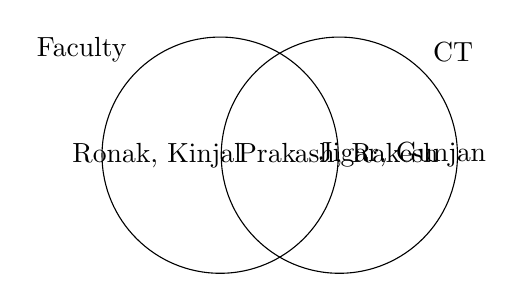
\begin{tikzpicture}
    \node[circle, draw, minimum size=3cm, label=135:Faculty] (fac) {};
    \node[circle, draw, minimum size=3cm, label=45:CT, right=-1.5cm of fac] (ct) {};
    
    \node at (fac) [xshift=-0.8cm] {Ronak, Kinjal};
    \node at (ct) [xshift=0.8cm] {Jigar, Gunjan};
    \node at (fac) [xshift=1.5cm] {Prakash, Rakesh}; 
\end{tikzpicture}
\end{center}

\end{solutionbox}

\begin{mnemonicbox}[title={UIMM}]Union Intersect Minus Minus\end{mnemonicbox}

\questionmarks{5(c) OR}{7}{Explain View Serializability in detail.}

\begin{solutionbox}

\textbf{View Serializability}: A schedule is view serializable if it is view equivalent to some serial schedule, meaning it produces the same "view" (or final state) of the database.

\textbf{Table: Comparison with Conflict Serializability}

\begin{table}[H]
    \centering
    \begin{tabulary}{\linewidth}{|L|L|L|}
    \hline
    \textbf{Aspect} & \textbf{View Serializability} & \textbf{Conflict Serializability} \\
    \hline
    Definition & Based on the final results of reads and writes & Based on conflicts between operations \\
    \hline
    Condition & Preserves initial read, final write, and read-write dependency & Preserves all conflicts between operations \\
    \hline
    Scope & Broader class of schedules & Subset of view serializable schedules \\
    \hline
    Testing & More complex to test & Can test with precedence graph \\
    \hline
    \end{tabulary}
\end{table}

\textbf{Diagram (Subset):}

\begin{center}
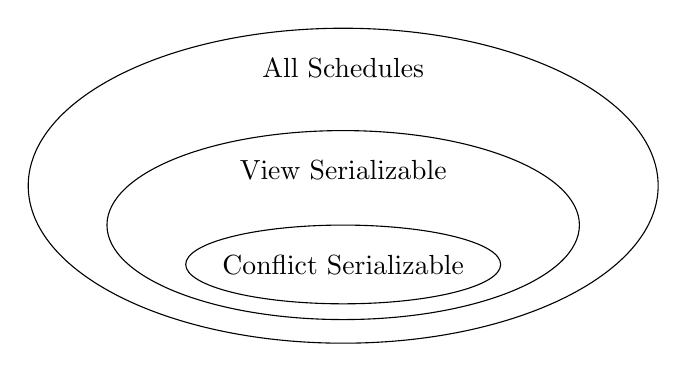
\begin{tikzpicture}
    \draw (0,0) ellipse (4cm and 2cm);
    \node at (0, 1.5) {All Schedules};
    
    \draw (0,-0.5) ellipse (3cm and 1.2cm);
    \node at (0, 0.2) {View Serializable};
    
    \draw (0,-1) ellipse (2cm and 0.5cm);
    \node at (0, -1) {Conflict Serializable};
\end{tikzpicture}
\end{center}

\textbf{View Equivalence Conditions:}
\begin{enumerate}
    \item Initial Reads: If T1 reads an initial value of data item A in schedule S1, it must also read the initial value in S2.
    \item Final Writes: If T1 performs the final write on data item A in S1, it must also perform the final write in S2.
    \item Read-Write Dependency: If T1 reads a value of A written by T2 in S1, it must also read the value written by T2 in S2.
\end{enumerate}

\textbf{Example of View Serializable but not Conflict Serializable Schedule:}
Consider transactions with blind writes (writes without reading):
\begin{itemize}
    \item T1: W1(A)
    \item T2: W2(A)
\end{itemize}
Schedule S: W1(A), W2(A) - View serializable to both T1$\rightarrow$T2 and T2$\rightarrow$T1 (final write is always T2)
But W1(A) and W2(A) conflict, so a conflict graph would have an edge in both directions.

\end{solutionbox}

\begin{mnemonicbox}[title={IRF}]Initial reads, Result writes, Final view\end{mnemonicbox}

\end{document}
